\documentclass{standalone}
\usepackage{tikz}
\usetikzlibrary{patterns}

\tikzset{
  svgfrag/.style 2 args={
    execute at begin scope={\special{dvisvgm:raw <g class="fragment #2" data-fragment-index="#1">}},
    execute at end scope={\special{dvisvgm:raw </g>}},
    execute at begin node={\special{dvisvgm:raw <g class="fragment #2" data-fragment-index="#1">}},
    execute at end node={\special{dvisvgm:raw </g>}},
  }
}

\begin{document}
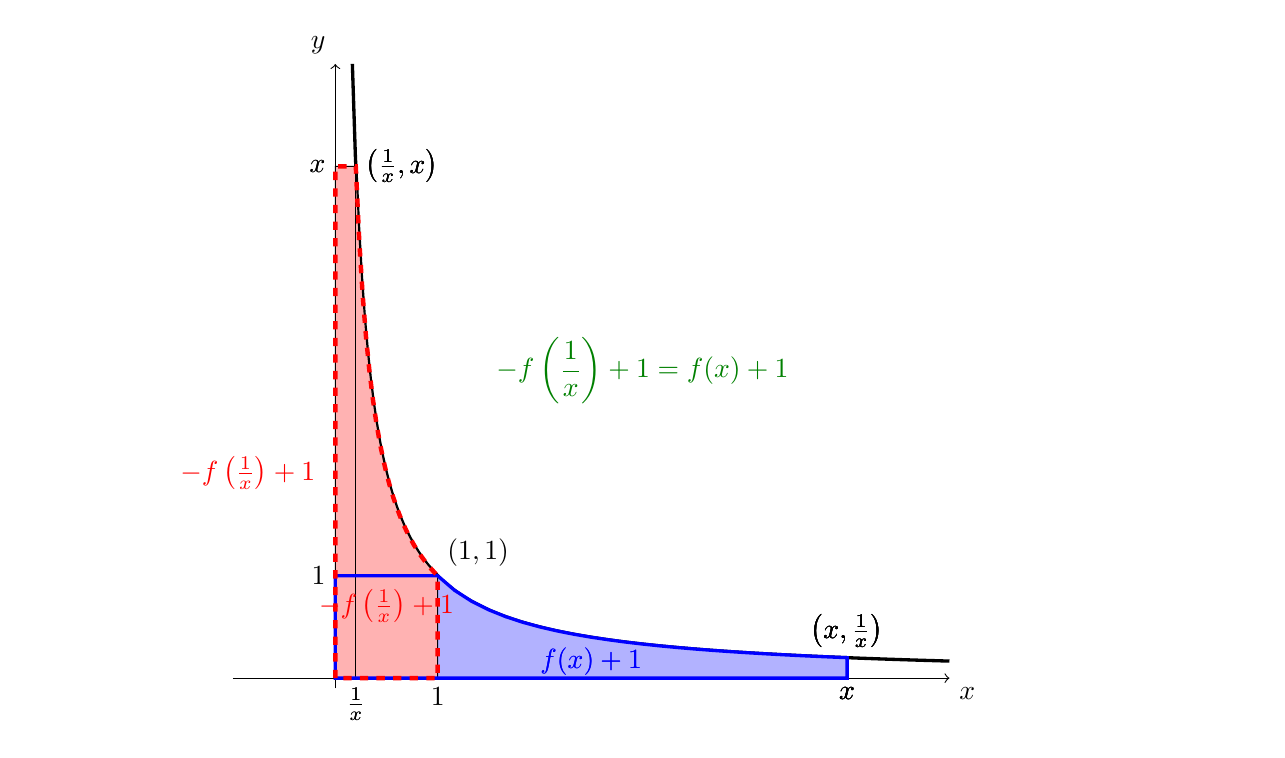
\begin{tikzpicture}[domain={1/6}:6, scale=1.3]
    \draw[white] (-3,-.2) rectangle (9,6.1);
    \draw[->] (-1,0) -- (6,0)node[below right]{$x$};
    \draw[->] (0, -.1) -- (0, 6)node[above left]{$y$};
    \draw[very thick] plot[samples=200] (\x, {1/\x});
    \draw[thin] (1,1)node[above right]{$(1,1)$} -- (1,0)node[below]{$1$};
    \begin{scope}[svgfrag={3}{fade-out}]
        \begin{scope}[svgfrag={1}{fade-in}]
            \draw[thin] (5,0.2)node[above]{$\left(x,\frac{1}{x}\right)$} -- (5,0)node[below]{$x$};
            \draw[thin, fill=blue!30!white, domain=1:5] (1,0) -- (1,1) --plot (\x, {1/\x}) -- (5,.2) -- (5,0) --cycle;
            \node[color=blue] at (3,1/6) {$f(x)$};
        \end{scope}
        \begin{scope}[svgfrag={2}{fade-in}]
            \draw[thin] (0.2, 5)node[right]{$\left(\frac{1}{x}, x\right)$} -- (0.2, 0)node[below]{$\frac{1}{x}$};
            \draw[thin, fill=red!30!white, domain=.2:1] (.2,0) -- (.2,5) --plot (\x, {1/\x}) -- (1,1) -- (1,0) --cycle;
            \node[color=red] at (.6,.7) {$-f\left(\frac{1}{x}\right)$};
        \end{scope}
    \end{scope}
    \begin{scope}[svgfrag={5}{fade-out}]
        \begin{scope}[svgfrag={3}{fade-in}]
            \draw[thin] (5,0.2)node[above]{$\left(x,\frac{1}{x}\right)$} -- (5,0)node[below]{$x$};
            \draw[thin] (1,1) -- (0,1)node[left]{$1$};
            \node at (.5,.5) {$1$};
        \end{scope}
        \begin{scope}[svgfrag={4}{fade-in}]
            \draw[thin] (5,0.2)node[above]{$\left(x,\frac{1}{x}\right)$} -- (5,0)node[below]{$x$};
            \draw[thin, fill=blue!30!white, domain=1:5] (0,0) -- (0,1) -- (1,1) --plot (\x, {1/\x}) -- (5,.2) -- (5,0) --cycle;
            \draw[thin] (1,1) -- (0,1);
            \node[color=blue] at (2.5,1/6) {$f(x) + 1$};
        \end{scope}
    \end{scope}
    \begin{scope}[svgfrag={7}{fade-out}]
        \begin{scope}[svgfrag={5}{fade-in}]
            \draw[thin] (0.2,5)node[right]{$\left(\frac{1}{x}, x\right)$} -- (.2,0)node[below]{$\frac{1}{x}$};
            \draw[thin] (0.2,5) -- (0,5)node[left]{$x$};
            \node at (0.1,2.5) {$1$};
        \end{scope}
        \begin{scope}[svgfrag={6}{fade-in}]
            \draw[thin, fill=red!30!white, domain=0.2:1] (0,0) -- (0,5) -- (0.2,5) --plot (\x, {1/\x}) -- (1,1) -- (1,0) --cycle;
            \draw[thin] (0.2,5) -- (.2,0);
            \node[color=red] at (.5,.7) {$-f\left(\frac{1}{x}\right) + 1$};
        \end{scope}
    \end{scope}
    \begin{scope}[svgfrag={7}{fade-in}]
        \draw[thin] (5,0.2)node[above]{$\left(x,\frac{1}{x}\right)$} -- (5,0)node[below]{$x$};
        \draw[very thick, blue, domain=1:5] (0,0) -- (0,1) -- (1,1) --plot (\x, {1/\x}) -- (5,.2) -- (5,0) --cycle;
        \node[color=blue] at (2.5,1/6) {$f(x) + 1$};
    \end{scope}
    \begin{scope}[svgfrag={8}{fade-in}]
        \draw[thin] (0.2,5)node[right]{$\left(\frac{1}{x}, x\right)$} -- (0,5)node[left]{$x$};
        \draw[ultra thick, red, dashed, domain=0.2:1] (0,0) -- (0,5) -- (0.2,5) --plot (\x, {1/\x}) -- (1,1) -- (1,0) --cycle;
        \node[color=red, left] at (-.1,2) {$-f\left(\frac{1}{x}\right) + 1$};
    \end{scope}
    \begin{scope}[svgfrag={9}{fade-in}]
        \node[color=green!50!black] at (3,3) {$\displaystyle -f\left(\frac{1}{x}\right) + 1 = f(x) + 1 $};
    \end{scope}
\end{tikzpicture}
\end{document}
